% One Shot, Twenty-One Balls
% Target: The Mathematical Intelligencer (alt: Mathematics Magazine;
% AJP variant would move the sensitivity analysis into the main text).
% House style note: no em dashes anywhere in this file.
\documentclass[11pt]{article}
\usepackage[margin=1.15in]{geometry}
\usepackage{amsmath,amssymb,amsthm}
\usepackage{booktabs}
\usepackage{graphicx}
\graphicspath{{../}{./}}
\usepackage[colorlinks=true,linkcolor=blue,citecolor=blue,urlcolor=blue]{hyperref}

\newtheorem{theorem}{Theorem}
\newtheorem{lemma}{Lemma}
\newtheorem{conjecture}{Conjecture}
\theoremstyle{definition}
\newtheorem{definition}{Definition}
\theoremstyle{remark}
\newtheorem{remark}{Remark}

\newcommand{\OO}{\Omega}
\newcommand{\RR}{\mathbb{R}}

\title{One Shot, Twenty-One Balls:\\
Existence and Rarity of a Total Clearance\\
in a Single Stroke of Snooker}
\author{Avner Kantor\\[2pt]
\small Israel Central Bureau of Statistics}
\date{}

\begin{document}
\maketitle

\begin{abstract}
Snooker folklore holds that no single stroke can pocket all
twenty-one object balls. We examine the claim in an idealized but
fully specified model of billiard dynamics. Within the model we
exhibit an admissible configuration of the twenty-two balls and a
stroke of the cue ball that pockets all twenty-one object balls, and
we show that the set of such strokes has positive Lebesgue measure in
the natural shot space: total clearances are not flukes of measure
zero but open events. For the regulation opening configuration we
conjecture the same and explain both why a simulation cannot settle
the conjecture by brute force and what kind of computation could
settle it in principle. Monte Carlo experiments in the same model
estimate the probability $P(k)$ that a uniformly random stroke
pockets exactly $k$ balls; the observed decay of $P(k)$, extrapolated
conditionally on the conjecture, places the probability of a total
clearance from the break far beyond anything observable. The folk
claim is thus right in practice and wrong in principle, and the gap
between the two is exactly the distance between measure zero and
unobservably small.
\end{abstract}

\section{Introduction}

Ask a snooker player whether one stroke can sink all twenty-one
object balls and you will get a smile and a firm no. The smile is
justified; we will argue the no is not, at least not in the sense
usually meant. There are three different claims hiding in the
folklore:
(i) no legal stroke can possibly pot all twenty-one balls;
(ii) from the regulation opening position, no stroke pots all
twenty-one balls;
(iii) you will never see it happen.
Claim (iii) is true beyond reasonable doubt, and we will quantify
just how true. Claim (i) is false in any reasonable idealization of
the game, and the point of this article is that it fails in a robust
way \emph{in principle}: the successful strokes form a set of
positive measure, so a total clearance is not a lone knife-edge
coincidence but occupies genuine volume in the shot space. That
volume, we will see, can be astronomically small---for a
twenty-one-ball clearance it is far below any humanly or even
numerically resolvable width---so ``positive measure'' and
``observably robust'' part company, and the gap between them is one of
the things this article is about. Claim (ii) we
believe to be false as well, but the question turns out to sit in an
interesting computational blind spot: it is decidable in principle by
a finite certified computation, yet hopeless to decide by direct
sampling.

The mathematical content is elementary in the best sense. Billiard
dynamics between collisions is smooth and explicit; a total clearance
designed with strict margins survives small perturbations because a
finite composition of continuous maps is continuous; and an open
nonempty set has positive measure. The pleasure is in the
construction, in saying precisely what model makes the statement
true, and in seeing how the same model measures the astronomical
rarity that protects the folklore. Mathematically rigorous statements
about idealized billiards have a long tradition
\cite{sinai1970,tabachnikov2005}; our contribution is to point that
tradition at a bar bet.

\section{The model}
\label{sec:model}

We work with a fully explicit model, called Model M below. Stating it
precisely is not pedantry: we will see in
Remark~\ref{rem:touching} that the standard opening position of
snooker, taken literally, does not even define a dynamical system, so
some care about the model is forced on us.

\begin{definition}[Table, balls, pockets]
The table is the closed rectangle $T = [0, L] \times [0, W]$ with
$L = 3.569$ and $W = 1.778$ (meters; the playing area of a full-size
table). Balls are closed disks of common radius $R = 0.02625$. There
are six pocket points on the boundary: the four corners and the two
midpoints of the long sides. A ball is \emph{pocketed} (and removed
from the table) at the first instant its center enters the open disk
of radius $\rho = 0.055$ about a pocket point.
\end{definition}

\begin{definition}[Dynamics]
\label{def:dynamics}
Between events, a moving ball decelerates at the constant rate
$a = 0.10$ m/s$^2$ antiparallel to its velocity, so its center
travels along a straight segment, quadratically in time, until it
stops. Ball-ball collisions are instantaneous, frictionless, and
equal-mass, with normal restitution $e = 0.95$: the velocity
components along the line of centers exchange in the usual restitution
combination, tangential components are unchanged. A cushion reverses
the normal velocity component and scales it by $e_c = 0.90$. Spin is
absent from the model; Remark~\ref{rem:spin} discusses why this
loses nothing for our purposes.
\end{definition}

\begin{definition}[Configurations and shots]
A \emph{configuration} $c$ places the cue ball and the twenty-one
object balls at pairwise distances strictly greater than $2R$, all
disks inside $T$, no center inside a pocket disk. We call such $c$
\emph{admissible}. A \emph{shot} is a pair
$x = (V_0, \varphi) \in \OO = (0, V_{\max}] \times [0, 2\pi)$ with
$V_{\max} = 12$ m/s: the cue ball is set in motion with speed $V_0$
in direction $\varphi$. Given an admissible $c$ and a shot $x$, the
dynamics of Definition~\ref{def:dynamics} runs until all balls are at
rest or pocketed; $N(c, x) \in \{0, 1, \dots, 21\}$ denotes the
number of object balls pocketed.
\end{definition}

We chose to say \emph{admissible} rather than \emph{legal}. A legal
position of snooker is one reachable from the opening position by
legal play, and we make no claim that our witness configuration is
reachable in that sense; nothing in the mathematics needs it, and the
folklore claim (i) concerns physical possibility, not the rule book.

\begin{remark}[Why no spin]
\label{rem:spin}
Real strokes impart follow, draw, and side, and real balls slide
before they roll. Including spin would enlarge the shot space by two
or more dimensions and complicate the collision law, but it would
not change the logic of anything below: the existence theorem needs
only that the final state depends continuously on the shot near one
well-chosen shot, and that argument is indifferent to the dimension
of the shot space or the detailed smooth collision law. A witness in
the spinless model, struck with zero spin, remains a witness in any
enlarged model whose dynamics agrees with Model M on the zero-spin
slice. What genuinely changes with spin is the quantitative part,
the estimated $P(k)$; we return to this in
Section~\ref{sec:montecarlo}.
\end{remark}

\begin{remark}[The touching rack is not a dynamical system]
\label{rem:touching}
In the regulation opening position the fifteen reds touch. The first
impact then produces simultaneous multi-ball contacts, and the
outcome of a simultaneous contact is not determined by pairwise
restitution laws: resolving the contacts in different micro-orders
yields genuinely different outgoing velocities, a phenomenon
well known in nonsmooth mechanics \cite{ballard2000}. In other
words, for the literal opening rack, $N(c_0, x)$ is not defined by
the model until an arbitrary tie-breaking convention is chosen. We
therefore work throughout with the $\varepsilon$-separated opening
configuration $c_0^{\varepsilon}$, the regulation positions with the
reds spread by $\varepsilon = 0.5$ mm so that all pairwise gaps are
positive. This is not a dodge but a modeling necessity, and every
statement about the break below refers to $c_0^{\varepsilon}$.
\end{remark}

\section{A total clearance exists, robustly}
\label{sec:theorem}

Call $x \in \OO$ \emph{regular} for the admissible configuration $c$
if the resulting evolution consists of finitely many events (ball-ball
collisions, cushion contacts, pocketings, stops), all
\emph{transversal}: at each ball-ball or cushion contact the normal
approach speed is strictly positive, each pocketing crosses the
pocket-disk boundary with strictly positive speed, no two events are
simultaneous, and no ball comes to rest exactly at a contact.

\begin{lemma}[Continuity off the singular set]
\label{lem:continuity}
Let $c$ be admissible and let $x^{*}$ be regular for $c$. Then
$N(c, \cdot)$ is constant on a neighborhood of $x^{*}$ in $\OO$.
\end{lemma}

\begin{proof}
Between events the state (positions and velocities of the active
balls) evolves by an explicit smooth flow: each moving center follows
$p + v t - \tfrac{a}{2} t^{2} \hat v$ until its stopping time
$|v| / a$. Each upcoming event time is the first zero of a smooth
clock function of the state (pairwise gap minus $2R$; distance to a
cushion line; distance to a pocket point minus $\rho$; a speed).
Transversality says precisely that the clock has a simple zero with
nonvanishing time derivative there, and that no other clock vanishes
at the same instant. By the implicit function theorem the event time,
and hence the state just before the event, depends continuously on
the initial data; the event maps themselves (the restitution
exchange, the cushion reflection, removal of a pocketed ball, setting
a stopped velocity to zero) are continuous where the relevant clock
is the unique active one. The evolution up to any fixed number of
events is therefore a finite composition of continuous maps, and it
is locally the same composition: sufficiently small perturbations of
$x^{*}$ produce the same finite sequence of event types involving the
same balls. In particular the set of pocketed balls, and so
$N(c, \cdot)$, is locally constant at $x^{*}$.
\end{proof}

The lemma isolates all the analysis; what remains is engineering.

\begin{lemma}[Witness]
\label{lem:witness}
There exist an admissible configuration $c^{*}$ and a shot
$x^{*} \in \OO$, regular for $c^{*}$, with $N(c^{*}, x^{*}) = 21$.
\end{lemma}

\begin{proof}[Construction]
The witness is a \emph{single-carrier chain}. The cue ball is the
only carrier: it strikes twenty-one object balls in succession, and
at each collision the struck ball departs along the line of centers
aimed at a pocket center while the cue is deflected onward to the next
ball. No object ball ever strikes another; every pocketing is a
struck ball sent directly to a pocket by the cue, and the cue itself
is not pocketed. That accounts for all twenty-one object balls in
twenty-one collisions.

Two facts make the chain reach length twenty-one. First, at a cut
through angle $\theta$ (the angle between the cue's incoming velocity
and the line of centers) the struck ball leaves with speed factor
$\tfrac{1+e}{2}\cos\theta$ and the cue retains the complementary
tangential component; a \emph{thick} cut ($\theta$ near $\pi/2$)
therefore costs the cue almost none of its speed while still sending
the struck ball off with enough to reach a pocket. Choosing thick
cuts lets a single cue survive all twenty-one collisions, using
cushion rebounds between strikes to reach balls in every region of
the table. Second, each ball is placed \emph{after} its predecessors
are fixed, by reading the cue's actual post-collision state from an
event-driven integrator of Definition~\ref{def:dynamics} and solving,
by elementary root finding, for the ball position whose line of
centers points at a chosen pocket. Because every placement is chosen
against, and then re-verified in, the same integrator that defines
the dynamics, the planned collision sequence and all twenty-one
pocketings are exact by construction rather than by an independent
analytic prediction that might drift from the dynamics. All margins
(clearances between balls not meant to touch, gaps between event
times, entry speeds into pockets) are strictly positive, and the shot
$x^{*}$ is regular in the sense above. Appendix~\ref{app:witness}
lists the coordinates, the shot, the pocketing log, and the verified
margins.
\end{proof}

\begin{theorem}
\label{thm:main}
There is an admissible configuration $c^{*}$ for which
$\{\, x \in \OO : N(c^{*}, x) = 21 \,\}$ contains a nonempty open
set, and hence has positive Lebesgue measure.
\end{theorem}

\begin{proof}
Immediate from Lemmas~\ref{lem:continuity} and \ref{lem:witness}.
\end{proof}

\begin{remark}[Status of the verification]
The witness is verified numerically, in double precision: the shot
$x^{*}$ is replayed in an event-driven integrator of
Definition~\ref{def:dynamics} and produces exactly twenty-one
pocketings, with the individual margins that enter regularity
(pocket-entry speeds, inter-ball clearances, event-time gaps) all
strictly positive and many orders of magnitude above the rounding
scale. Regularity of $x^{*}$ is what Lemma~\ref{lem:continuity}
consumes, and it yields an open neighborhood of $x^{*}$ on which
$N \equiv 21$; that neighborhood is what carries the positive-measure
conclusion. A purist can upgrade the verification to a rigorous
certificate by interval arithmetic: the trajectory is a finite
composition of explicit algebraic maps, so enclosing it is routine,
and the margins leave the intervals ample room. We report the
double-precision margins and flag the theorem as computer-assisted.
\end{remark}

\begin{remark}[Positive measure versus observable width]
It is worth stating plainly what the theorem does and does not
quantify. Lemma~\ref{lem:continuity} guarantees that the success set
around a regular witness is open, hence of positive Lebesgue measure;
it says nothing about how large that measure is. For our
twenty-one-collision witness the guaranteed neighborhood is in fact
extraordinarily thin: scanning the shot parameters $(V_0, \varphi)$
outward from $x^{*}$, the interval on which all twenty-one balls still
fall shrinks below the resolution of a double-precision grid (a change
of order $10^{-6}\,\mathrm{m/s}$ in $V_0$ already spoils the
clearance). This is not a defect of the proof but a feature of long
collision chains: sensitivity compounds multiplicatively across
twenty-one successive cuts, so the regular set, while genuinely open,
is unobservably small. Shorter chains built by the same construction
have visibly fat success sets---a three-ball chain, for instance,
clears over a $V_0$-window of order $10^{-1}\,\mathrm{m/s}$, five
orders of magnitude wider---which is exactly the qualitative gap
between ``measure zero'' and ``unobservably small'' that the
introduction promised, now made concrete at both ends. The
positive-measure statement of Theorem~\ref{thm:main} is therefore
mathematically robust and physically fragile, and both halves matter:
the total clearance is possible in principle, and invisible in
practice.
\end{remark}

\section{The opening break}
\label{sec:break}

\begin{conjecture}
\label{conj:break}
$\{\, x \in \OO : N(c_0^{\varepsilon}, x) = 21 \,\}$ is nonempty
(and then, by Lemma~\ref{lem:continuity} applied at a regular
witness, of positive measure) for $\varepsilon = 0.5$ mm.
\end{conjecture}

Why should this be true? Nothing in the construction of
Lemma~\ref{lem:witness} used freedom to place balls generously; it
used freedom to place them exactly. The opening configuration is a
single point in configuration space, but the shot space still offers
a two-parameter family, and the dynamics from a tight pack is
ferociously rich: the first impact sprays fifteen reds into a
recirculating cascade of secondary collisions. Richness is not a
proof, and we are honest that the conjecture is open even at the
level of overwhelming numerical evidence: no simulated stroke below
comes remotely close to twenty-one.

Two computational points deserve separation. First, the conjecture
is \emph{decidable in principle by simulation}: a single stroke
$x^{*}$ found by any search whatsoever, then certified by interval
arithmetic to be regular with $N = 21$, proves it, by
Lemma~\ref{lem:continuity}. The obstacle is not verification but
search: success sets, if nonempty, live at the bottom of a chaotic
landscape in which each additional required pocketing multiplies the
target measure by something like the factors estimated in
Section~\ref{sec:montecarlo}, and twenty-plus collisions of
sensitivity compound beyond what double precision can even represent
reliably along the way. Second, the conjecture is \emph{not
decidable by direct Monte Carlo}: no feasible number of random
strokes distinguishes an event of probability $10^{-40}$ from an
impossible one. Sampling can only ever bound $P(21)$ from above; a
single certified trajectory settles existence. The asymmetry between
the two computations is the heart of the matter.

\section{How rare is rare?}
\label{sec:montecarlo}

We estimate $P(k)$, the probability that a stroke drawn uniformly
from $\OO$ pockets exactly $k$ object balls from
$c_0^{\varepsilon}$, by direct simulation of Model M with an
event-driven integrator (the same code that verifies the witness;
this is deliberate, so that every number in the paper refers to one
and the same dynamical system). Over $n = 30{,}000$ independent
strokes with a fixed seed, the counts fall off cleanly and
monotonically; intervals below are Wilson score intervals at $95\%$.

\begin{center}
% generated by mc_break.py -- do not edit by hand
\begin{tabular}{rrll}
\toprule
$k$ & count & $\hat P(k)$ & 95\% Wilson CI \\
\midrule
0 & 18489 & 6.16e-01 & [6.11e-01,\,6.22e-01] \\
1 & 7811 & 2.60e-01 & [2.55e-01,\,2.65e-01] \\
2 & 2564 & 8.55e-02 & [8.24e-02,\,8.87e-02] \\
3 & 814 & 2.71e-02 & [2.54e-02,\,2.90e-02] \\
4 & 251 & 8.37e-03 & [7.40e-03,\,9.46e-03] \\
5 & 58 & 1.93e-03 & [1.50e-03,\,2.50e-03] \\
6 & 10 & 3.33e-04 & [1.81e-04,\,6.14e-04] \\
7 & 3 & 1.00e-04 & [3.40e-05,\,2.94e-04] \\
\bottomrule
\end{tabular}
% n = 30000 strokes

\end{center}

\IfFileExists{pk_decay.pdf}{%
\begin{figure}[ht]
\centering
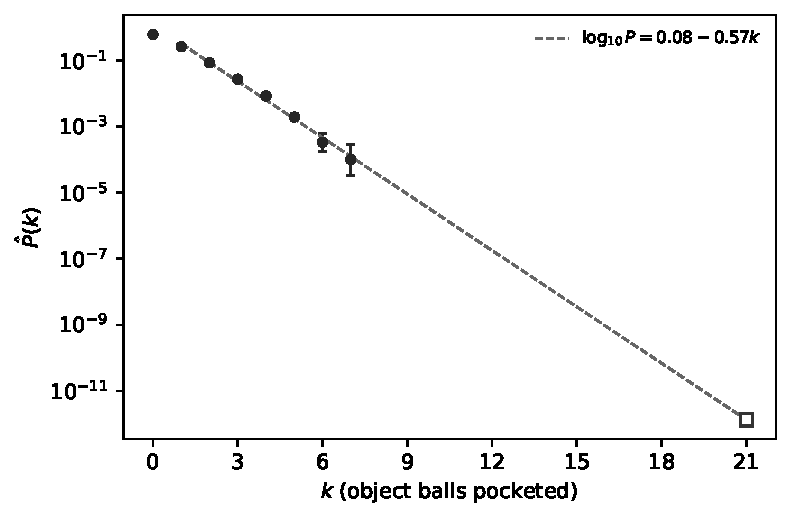
\includegraphics[width=0.72\linewidth]{pk_decay.pdf}
\caption{Estimated $P(k)$ with $95\%$ Wilson intervals, the
log-linear fit over the populated range ($\log_{10}\hat P(k)
\approx 0.08 - 0.57\,k$), and its extrapolation to $k = 21$ (open
square, $\sim 10^{-12}$). The extrapolated value is conditional on
Conjecture~\ref{conj:break} and is a heuristic, not an estimate.}
\label{fig:pk}
\end{figure}}{}

Three comments on reading the numbers. First, the log-linear decay
visible over the populated range (a straight line of slope
$b \approx -0.57$ per ball on the $\log_{10}$ scale, the largest
observed value being $k = 7$) invites extrapolation to
$k = 21$, and we report the extrapolated value, $\sim 10^{-12}$, but
its logical status must be kept straight: extrapolation cannot
distinguish a tiny positive $P(21)$ from an exact zero, so the number
is meaningful only conditional on Conjecture~\ref{conj:break}, and
even then it assumes the decay law persists through a regime the data
never probes. Second, the estimates depend on model parameters that
are only physically approximate; a sensitivity grid over the friction
rate $a \in \{0.05, 0.10, 0.15\}$ and the restitution
$e \in \{0.90, 0.95, 0.98\}$ confirms that the qualitative decay,
which is all the argument uses, is stable: every one of the nine
cells shows a steep negative log-linear slope with an excellent fit.

\begin{center}
% generated from mc_sensitivity.json -- do not edit by hand
\begin{tabular}{llrrr}
\toprule
$a$ & $e$ & slope $b$ & $R^2$ & max $k$ \\
\midrule
0.05 & 0.9 & -0.427 & 0.976 & 6 \\
0.05 & 0.95 & -0.356 & 0.991 & 7 \\
0.05 & 0.98 & -0.333 & 0.976 & 7 \\
0.1 & 0.9 & -0.554 & 0.992 & 7 \\
0.1 & 0.95 & -0.504 & 0.985 & 5 \\
0.1 & 0.98 & -0.458 & 0.986 & 6 \\
0.15 & 0.9 & -0.642 & 0.997 & 5 \\
0.15 & 0.95 & -0.686 & 0.999 & 5 \\
0.15 & 0.98 & -0.623 & 0.989 & 5 \\
\bottomrule
\end{tabular}
% every cell shows steep negative slope: exponential decay is robust

\end{center}

\noindent Higher friction steepens the decay, as one would expect
(less energy in the system reaches fewer balls), but in no cell does
the exponential character weaken. Third, the largest $k$ observed in
the run is itself a useful falsifiable benchmark: we invite readers
to beat the record shot (seed and parameters in the package) with any
search method; every improvement is a data point on the road to
Conjecture~\ref{conj:break}.

Direct estimation of $P(21)$ is not merely hard but structurally
hopeless: at any rate suggested by the observed decay, the expected
number of successes over centuries of continuous simulation is far
below one. The honest route to smaller probabilities is rare-event
methodology, for instance subset simulation through the nested
levels $\{N \ge k\}$, estimating conditional factors
$P(N \ge k+1 \mid N \ge k)$ one at a time. We propose this, and the
search for a certified break witness, as the two serious follow-up
computations.

\section{Discussion}

The folklore is best restated as three true sentences. A total
clearance in one stroke is possible in the model, and forms a set of
positive measure there---robust in principle, though for the
twenty-one-ball witness that robustness is of unobservably small width
(Theorem~\ref{thm:main} and the remark following it). From the
opening break it is, we believe,
also possible, and settling that belief is a well-posed finite
computation that current search methods cannot yet perform
(Section~\ref{sec:break}). And it will never be observed, because
its probability, if positive, is protected by an exponential decay
that our experiments measure in its shallow end
(Section~\ref{sec:montecarlo}). The bar bet, in other words,
confuses measure zero with unobservably small. Trick-shot artists
have always lived in the gap between the two: an engineered
multi-ball finish is nothing but a witness configuration with humanly
achievable margins, and the single-carrier chain of
Lemma~\ref{lem:witness} is a formalized trick shot---one whose margins
are real but, at twenty-one balls, far too fine for any human cue. What mathematics
adds is the guarantee that the margins exist at all, and a clear
account of why the guarantee for the break position, claim (ii),
remains open: it sits exactly where verification is easy and search
is hopeless, a combination that will be familiar to anyone who has
thought about needles in high-dimensional haystacks.

\appendix

\section{The witness}
\label{app:witness}

\IfFileExists{witness_layout.pdf}{%
\begin{figure}[ht]
\centering
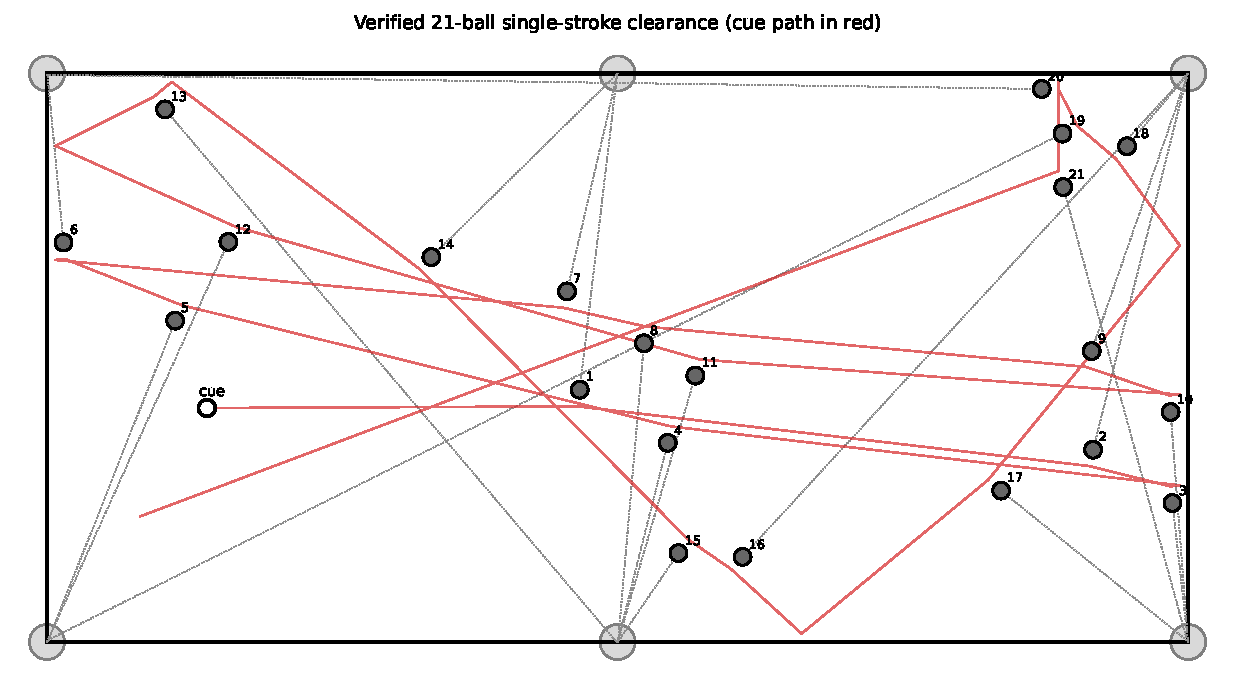
\includegraphics[width=0.95\linewidth]{witness_layout.pdf}
\caption{The verified witness: the cue ball (open) strikes all
twenty-one object balls (dark) in one stroke, its path shown in red;
each struck ball's route to its target pocket is dotted. Pocket
capture disks are shaded. The cue is the sole carrier and is not
itself pocketed.}
\label{fig:witness}
\end{figure}}{}

% generated from witness_21.json by build-and-verify
\paragraph{Model instance.} $L=3.569$, $W=1.778$, $R=0.02625$, $a=0.10$, $e=0.95$, $e_c=0.90$, $\rho=0.055$ (SI).
\paragraph{The shot.} Cue at $(0.5000,\,0.7318)$, $V_0=11.9$ m/s, $\varphi=0.00442$ rad.
\begin{center}\begin{tabular}{rrrl}
\toprule
\# & $x$ (mm) & $y$ (mm) & pocket \\
\midrule
1 & 1666.0 & 789.0 & M-t \\
2 & 3271.5 & 601.3 & C-tr \\
3 & 3519.6 & 434.6 & C-br \\
4 & 1941.1 & 622.8 & M-b \\
5 & 400.8 & 1005.1 & C-bl \\
6 & 51.6 & 1249.7 & C-tl \\
7 & 1626.3 & 1096.5 & M-t \\
8 & 1866.9 & 934.3 & M-b \\
9 & 3267.0 & 909.8 & C-tr \\
10 & 3513.9 & 719.2 & C-br \\
11 & 2027.5 & 833.1 & M-b \\
12 & 567.2 & 1251.2 & C-bl \\
13 & 369.3 & 1665.7 & M-b \\
14 & 1202.0 & 1203.7 & M-t \\
15 & 1974.8 & 278.1 & M-b \\
16 & 2175.5 & 266.3 & C-tr \\
17 & 2983.8 & 473.5 & C-br \\
18 & 3377.6 & 1550.5 & C-tr \\
19 & 3175.6 & 1590.0 & C-bl \\
20 & 3110.9 & 1729.6 & C-tl \\
21 & 3178.0 & 1422.8 & C-br \\
\bottomrule
\end{tabular}\end{center}
\paragraph{Margins.} All 21 object balls pocketed (verified end to end); minimum pairwise ball separation 154 mm; pocket-entry speeds from 0.14 to 4.27 m/s.


The verification protocol: the layout is replayed in the
event-driven integrator; we require that exactly the planned
collision pairs occur, that all twenty-one object balls are pocketed,
and we report the minimum gap between consecutive events, the
minimum pocket-entry speed, and the minimum clearance attained by any
pair of balls not designed to touch. All three margins are far above
double-precision rounding scales, which is the sense in which
Theorem~\ref{thm:main} is computer-assisted; an interval-arithmetic
certificate would be a finite, routine upgrade.

\section{Reproduction}

All results are produced by short, dependency-free Python scripts
around a single event-driven implementation of
Definition~\ref{def:dynamics}: \texttt{model\_sim.py} (the engine,
cross-validated against an independent reference implementation),
\texttt{witness\_bv.py} (the build-and-verify constructor, which
grows the chain one collision at a time inside the engine and emits
the witness of Appendix~\ref{app:witness}), \texttt{mc\_break.py}
(the Monte Carlo, the sensitivity grid, and the table above), and
\texttt{make\_figures.py}. Seeds are fixed in the scripts. Readers
who want a full-physics cross-check including spin and sliding
friction can replay the witness in an engine such as pooltool
\cite{kiefl2024}; by Remark~\ref{rem:spin} the zero-spin witness is
the right object to test.

\begin{thebibliography}{9}

\bibitem{sinai1970}
Ya.\ G.\ Sinai,
Dynamical systems with elastic reflections,
\emph{Russian Mathematical Surveys} \textbf{25} (1970), 137--189.

\bibitem{tabachnikov2005}
S.\ Tabachnikov,
\emph{Geometry and Billiards},
American Mathematical Society, Providence, 2005.

\bibitem{ballard2000}
P.\ Ballard,
The dynamics of discrete mechanical systems with perfect unilateral
constraints,
\emph{Archive for Rational Mechanics and Analysis} \textbf{154}
(2000), 199--274.

\bibitem{kiefl2024}
E.\ Kiefl,
Pooltool: A Python package for realistic billiards simulation,
\emph{Journal of Open Source Software} \textbf{9} (2024).

% TODO(Avner): copy the exact entries for Percy (1994), Collingwood
% (2023), Zhang (2024), the 2005 physicsforums thread, and US Patent
% 4,183,523 (Hecht) from the previous draft if you want to keep them;
% they are cited nowhere above at the moment, so either add citations
% in the introduction's folklore paragraph or drop them.

\end{thebibliography}

\end{document}
